\documentclass[11pt]{beamer}
\usepackage{verbatim}
\usepackage{amsmath}
\usepackage{amsthm}
\usepackage{multicol}
\usepackage{graphics}
\usepackage{color}
\usepackage{stmaryrd}\usefonttheme[onlymath]{serif}

\title{Automatic Loop Summarization via Path Dependency Analysis}
\date{\today}
\author{Xiaofei Xie et al.}


\begin{document}
\maketitle
\begin{frame}\frametitle{Overview of the paper}

\begin{itemize}
\item Introduction to loop summary and its application.
\item Path dependency automaton and basic thought of using it for summarizing.

\item Loop analysis and construction of PDA.
\item Summarization of different kinds of loops.

\item Experimental results.
\end{itemize}
\end{frame}
\begin{frame}\frametitle{Contributions}
\begin{itemize}
\item Propose a path dependency automaton to model the relatioships betwen paths of loops.
\item Propose classification defines what types of multi-path loops we can handle.
\item Develop the tool \textsc{Proteus} for loop summarization.
\end{itemize}
\end{frame}
\begin{frame}\frametitle{Introduction to Loop Summary}
Loop summary captures the relationship between the inputs and outputs of a loop as a set of symbolic constraints.

This means that the summary of a loop is a $\phi(X, X')$ s.t. ...
\textbf{Applications:}
\begin{itemize}
\item Loop bound analysis.
\item Program verification. $\models\phi(X, X') \wedge \neg p$.
\item Test case generation.

\end{itemize}
\end{frame}

\begin{frame}\frametitle{Path Dependency Automaton}
\begin{definition}[PDA]
Given a loop with its CFG $\mathcal{G} = (L, E, l_{pre}, L_h, L_e)$, the path dependency automaton is a tuple $\mathcal{A} = (Q, \mathcal{L}, q_0, accept, T)$, where
\begin{itemize}
\item $Q$ is a finite set of states.
\item $\mathcal{L}: Q\rightarrow \Pi_\mathcal{G}$. We use $\mathcal{L}_q$ to represent $\mathcal{L}(q)$.
\item $T = \{(q, q')\in Q\times Q\mid tail(\mathcal{L}_q) = head(\mathcal{L}_{q'}) \wedge \mathcal{L}_q \neq \mathcal{L}_{q'} \wedge (\exists k: (\bigwedge_{0 \le i  < k} \theta_{\mathcal{L}_q}[X_{\mathcal{L}_{q^i}}/X]) \wedge \theta_{\mathcal{L}_{q'}}[X_{\mathcal{L}_{q^k}}/ X])$ is satisfiable $\}$  is a finite set of transitions.
\end{itemize}
\end{definition}
\end{frame}
\begin{frame}\frametitle{Feasible Traces}
\begin{definition}[Traces]
Given a loop with its PDA $\mathcal{A} = (Q, \mathcal{L}, q_0, accept, T)$, $E_\mathcal{A} = \{(q_0, \ldots, q_n)\mid q_n\in accept \wedge \exists k_0, \ldots, k_{n-1}:\bigwedge_{0 \le i < n }((\bigwedge_{0 \le j < k_i}\theta_{\mathcal{L}_{q_i^j}}[X_{\mathcal{L}_{q_i^j}}/ X]) \wedge \theta_{\mathcal{L}_{q_i + 1}}[X_{\mathcal{L}_{q_i^{k_i}}}/ X])\}$ is satisfiable, where $X_{\mathcal{L}_{q_0^0}} = X\wedge \forall 0 < i \le n: X_{\mathcal{L}_{q_i^0}} = X_{\mathcal{L}_{q_{i - 1}^{k_{i - 1}}}}\}$ is the set of feasible traces.

\end{definition}

\end{frame}
\begin{frame}\frametitle{Loop Summarization}
\begin{definition}[Loop summary]
Given a PDA $\mathcal{A}$ and a set of variables $X$, the summary of a trace $\tau\in E_\mathcal{A}$ is the constraints denoted as $\phi(X, X_\tau)$.

The disjunctive loop summary(DLS) of $\mathcal{A}$, denoted as $S_\mathcal{A}$ is $\bigvee_{\tau\in E_\mathcal{A}}\{\phi(X, X_\tau)\}$.
\end{definition}


Problem: What if the set $E_\mathcal{A}$ is infinite?

We have to analysize the loop to find out:
\begin{itemize}
\item Whether $E_\mathcal{A}$ is infinite?
\item If it is infinite, whether we can inductively generate the DLS?

\end{itemize}
In order to inductively generate DLS, we need to specify the variables, loop conditions and different types of path interleaving.
\end{frame}

\begin{frame}\frametitle{Patterns of Value Changes and Path Conditions}

\begin{definition}[$n$-$th$ Term of Variable]
Given a variable $x $ and an iterative  path $\sigma$, the $n$-$th$ term of the variable $x$ in the path $\sigma$ is the value of $x$ after $n$ consecutive execution of $\sigma$.

\end{definition}

\begin{example}
If the $x$ is an arithmetic update, we can compute $x_n = x_0 + n*d$ where $x_0$ is the initial value of $x$ and $d$ is the common difference of variable $x$.
\end{example}
\end{frame}

\begin{frame}\frametitle{Criterias of Variables}
\begin{definition}[IV, MIV, NIV]\
\begin{itemize}

\item A variable $x$ is an induction variable(IV) in a path $\sigma$ if the value of $x$ after $n$ consecutive execution of $\sigma$ can be computed with the initial value $x_0$ and the number of iteration $n$.

\item Specifically, $x$ is a monotonic induction variable(MIV) in a path if $x$ is an IV and the value of $x$ is strictly monotonic.

\item Otherwise, we call the variable a non-induction variable(NIV).

\end{itemize}


\end{definition}
\begin{example}
\begin{itemize}

\item \texttt{for}($x <= n$)$\{x := x + 1;\}$ here $x$ is a (M)IV.

\item \texttt{for}($x[0] <= n$)$\{x[1] := x[1] + 1;\}$. Here $x[0]$ is a NIV for it is a nondeterministic value in the array.
\end{itemize}

\end{example}
\end{frame}


\begin{frame}\frametitle{Patterns of Path Interleaving}
\begin{itemize}
\item Sequential Execution. There is no cycle in each trace $\tau\in E_\mathcal{A}$.
\item Periodic Execution. If all the cycles in every trace are  periodic.
\item Irregular Execution. Otherwise.
\end{itemize}
\end{frame}

\begin{frame}\frametitle{Classification of the Loop}
Based on the different patterns of variables, conditions and path interleaving, a classification of the loop is given below.
\begin{center}
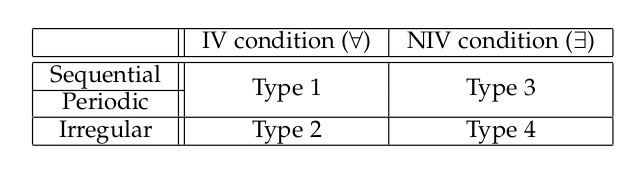
\includegraphics[scale=0.4]{classification.png}
\end{center}
\end{frame}

\begin{frame}\frametitle{Examples of Different Types of Loops}
\begin{multicols}{2}

\textbf{Type1 loop:}
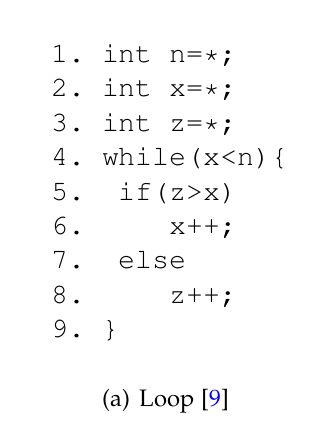
\includegraphics[scale=0.3]{type1exp.png}
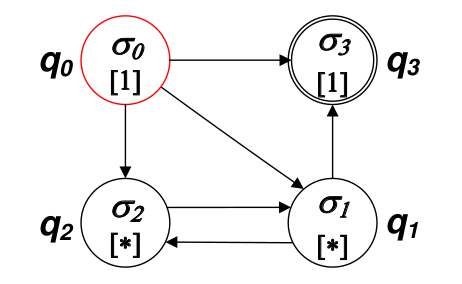
\includegraphics[scale=0.3]{type1pda.png}
This example is a type 1 loop:
\begin{itemize}
\item The variables are inductive variables and so are the conditions.
\item Loop in the PDA $(q_1, q_2)$ is a periodic loop.
\end{itemize}
\end{multicols}
\end{frame}

\begin{frame}\frametitle{Examples of Different Types of Loops}
\begin{center}
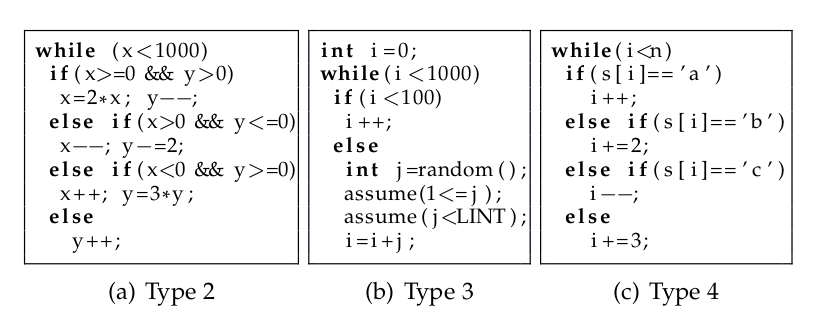
\includegraphics[scale=0.35]{othertypeexp.png}
\end{center}
\begin{itemize}
\item Type 2: variables are IVs but the interleaving of all the branches are irregular.

\item Type 3: variables include NIVs for j is dependent on \texttt{random()}, the execution is sequential from \texttt{if} branch to \texttt{else} branch.

\item Type 4: conditions includes arrays and hence is NIVs. The array also induces the irregular transition of the branches.  
\end{itemize}

\end{frame}

\begin{frame}\frametitle{Overview of the Tool: \textsc{•}{Proteus}}
\begin{center}
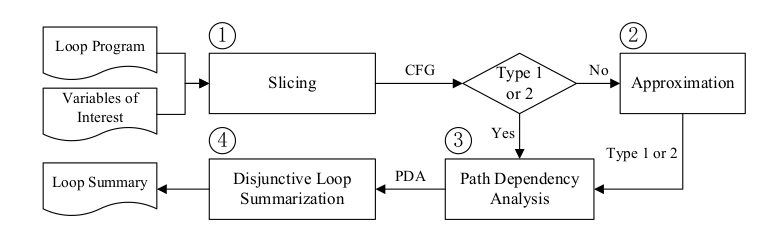
\includegraphics[scale=0.4]{proteus.png}
\end{center}
As shown by the flow graph, the tool first slice the program to find the loops together with the variables of interest.

After obtaining the loops from slicing, we use above types definition to categoritze them into respective types.

Then construct PDA and do disjunctive loop summarization.


\end{frame}

\begin{frame}\frametitle{PDA Construction: Slicing}
Loop slicing is based on the program dependence graph that combines control flow dependencies and data flow dependencies. 

It is targeting on reducing irrelevant paths in the constructed CFG and make summarization more efficient.

\begin{example}[Slicing]
\begin{center}
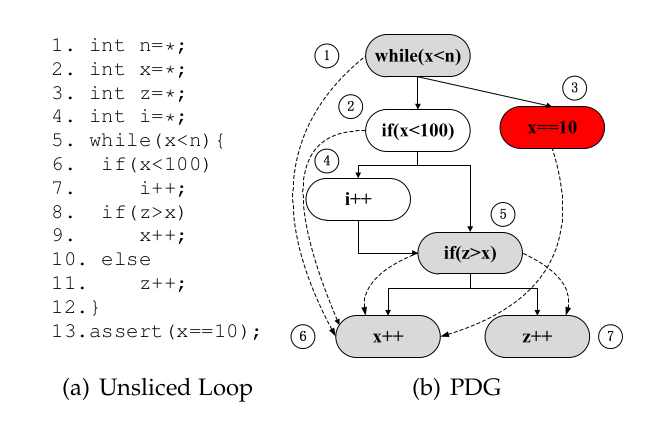
\includegraphics[scale=0.29]{slicing.png}
\end{center}
\end{example}

Control flow dependency(solid arrow).Data flow dependecy(dotted arrow).
\end{frame}

\begin{frame}\frametitle{PDA Construction: Computing $n$-$th$ Term in a Loop}
To compute the $n$-$th$ term computation, we consider the following two kinds of sequences:
\begin{itemize}
\item Basic sequence: Arithmetic sequence ($x_n = x_0  + c \times n$), geometric sequence ($x_n = x_0 \times c^n$) and constant sequence.

\item Dependent sequence: if a sequence depends on another sequence. e.g. $x_n = x_{n - 1} + y_n, x_n =x_{n - 1} \times y_n$.
\end{itemize}
Based on these two kinds of sequence, we can compute value after $n$-$th$ execution of the loop. 
\end{frame}


\begin{frame}\frametitle{PDA Construction}
\begin{center}
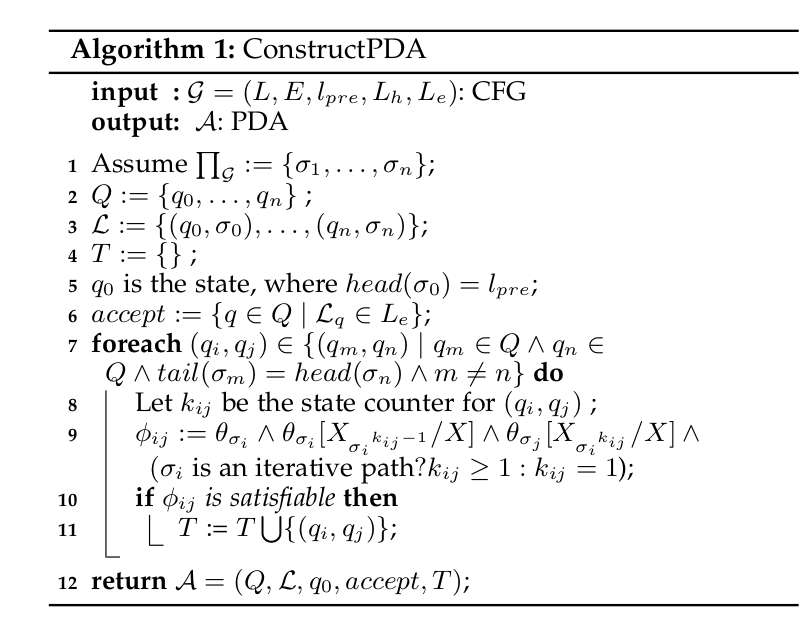
\includegraphics[scale=0.26]{algo1.png}
\end{center}
\begin{theorem}
If $\phi_{ij}$ in Algorithm is satisfiable, then $q_i$ can transit to $q_j$.
\end{theorem}
\end{frame}


\begin{frame}\frametitle{Examples and Structure of the Loops}

\begin{center}
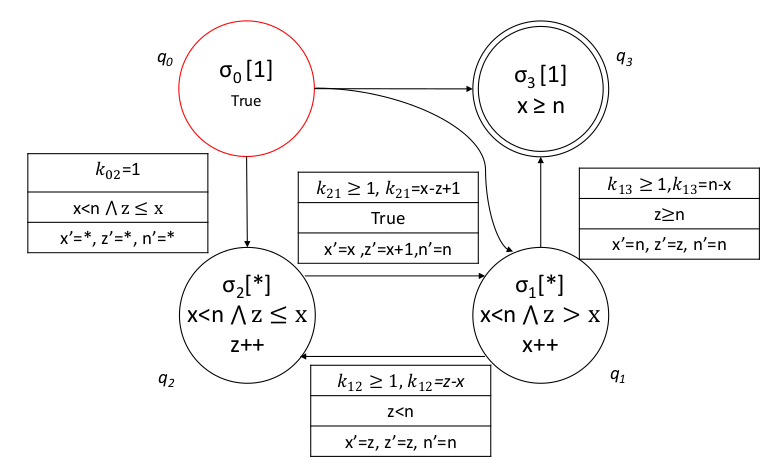
\includegraphics[scale=0.3]{loopdetail.png}

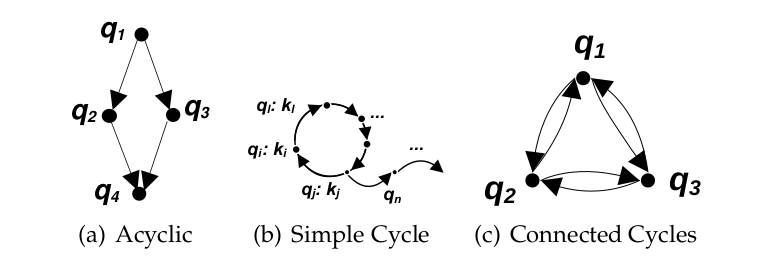
\includegraphics[scale=0.3]{pdaloops.png}
\end{center}
\end{frame}

\begin{frame}\frametitle{Summarization of Acyclic PDA}
\textbf{Summarization for type 1 acyclic PDA:}

Varibles are IVs and all traces can be traversed.

\begin{center}
\begin{center}

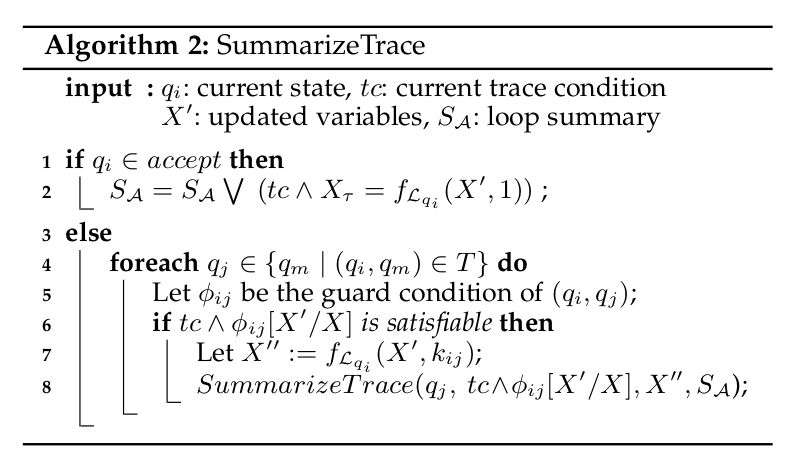
\includegraphics[scale=0.36]{algo2.png}
\end{center}
\end{center}
\end{frame}

\begin{frame}\frametitle{Example of Acyclic PDA}
If we ignore transition between $q_1$ and $q-2$.
\begin{center}

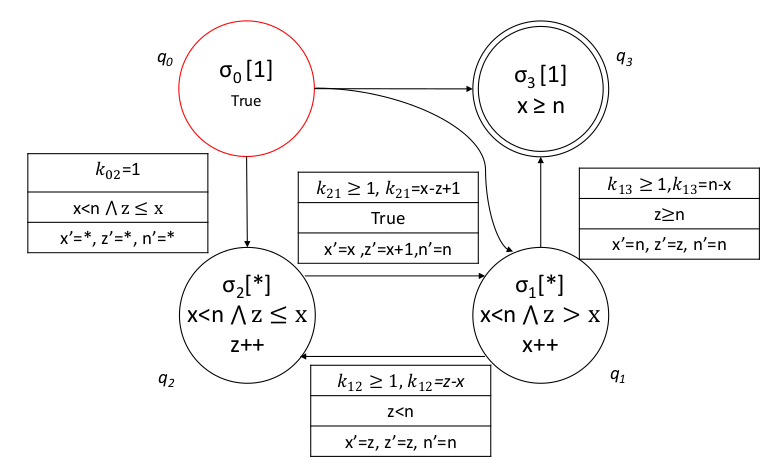
\includegraphics[scale=0.3]{loopdetail.png}
\end{center}
\end{frame}
\begin{frame}\frametitle{Summarization of PDA}
\textbf{Summarization for type 1 loops with simples cycles}

Difficulty: the execution count of the loop is uncertain.

But if the variables are updated regularly in the cycle, we can reduce the cycle into one state.

Determine periodic cycle (IV conditions and IV state counters): 

For a cycle $c = (q_l, q_{l+1}, \ldots, q_i)$, it can be regarded as $q_c$ in the PDA.

We use $k_n$ to represent the state counter from $q_n\in c$ to its successor in the cycle. Then the path condition can be represented as

\[\theta_{\mathcal{L}_{q_c}} = \theta_{\mathcal{L}_{q_l}} \wedge \theta_{\mathcal{L}_{q_{l+1}}}[f_{\mathcal{L}_{q_l}}(X, k_l)/X] \wedge \cdots \]\[\wedge \theta_{\mathcal{L}_{q_i}}[f_{\mathcal{L}_{q_i - 1}}(\ldots(f_{\mathcal{L}_{q_l}}(X, k_l))\ldots, k_{i-1})/X]\]
\end{frame}


\begin{frame}\frametitle{Summarization of PDA}
Besides, a cycle may have several outports. We find the state that may exit the cycle and use the summarization of acyclic PDA to summarize the rest part.


\begin{center}
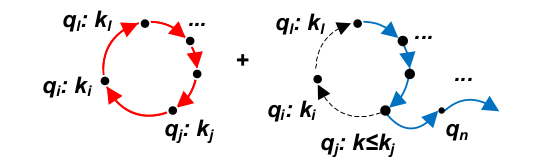
\includegraphics[scale=0.4]{partial.png}
\end{center}
\end{frame}
\begin{frame}\frametitle{Summarization of Periodic Cycles}

\begin{center}
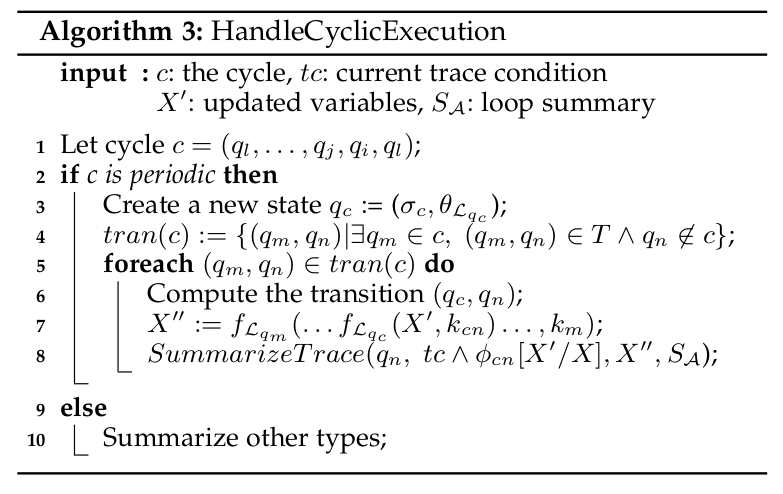
\includegraphics[scale=0.35]{algo3.png}
\end{center}
Here $k_i$s are from the summary in the subtrace $(q_l, q_{l+1}, \ldots, q_{l})$.
\end{frame}

\begin{frame}\frametitle{Example}
\begin{center}
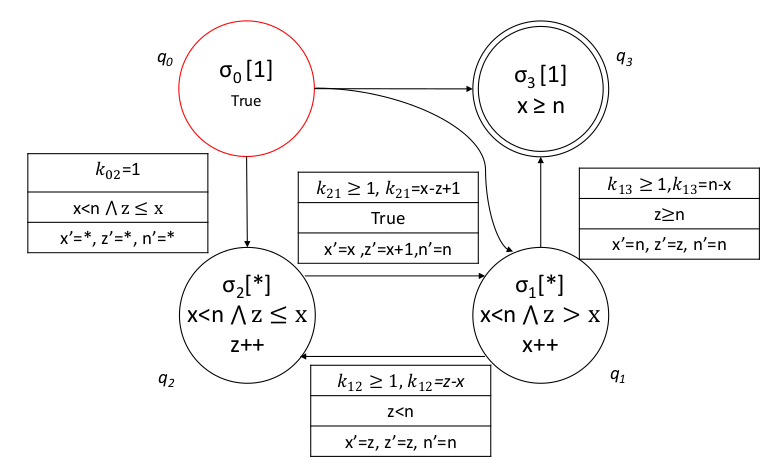
\includegraphics[scale=0.2]{loopdetail.png}

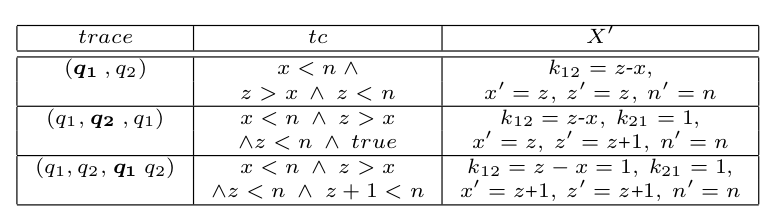
\includegraphics[scale=0.35]{tracetable.png}

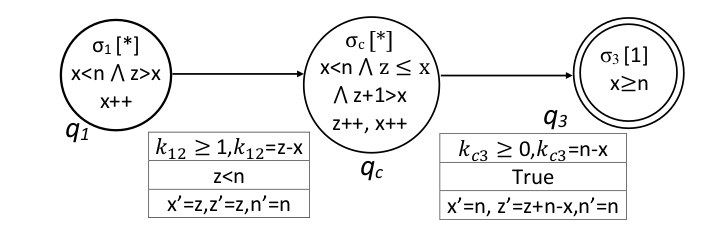
\includegraphics[scale=0.3]{merged.png}
\end{center}
\end{frame}

\begin{frame}\frametitle{Summarization for PDA with Connected Cycles}
\begin{center}

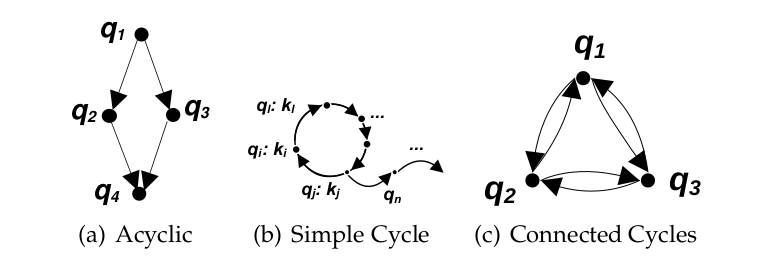
\includegraphics[scale=0.3]{pdaloops.png}
\end{center}

It it non-trivial to summarize connected cycles. Take above $(c)$ as an example.

Idea: We can compute the dependency between cycles. If the execution of the cycles are sequential under certain precondition, we can summarize the loop by summarizing a sequence of simple cycles.
\end{frame}

\begin{frame}\frametitle{Soundness}
\begin{theorem}
Given a Type 1 loop with the PDA
$\mathcal{A}$ and the summary $\bigcup_{\tau\in E_\mathcal{A}} \{\phi(X, X_\tau)\}$ , the summarized
constraints $\phi(X, X_\tau)$ for each trace $\tau$ are satisfiable after
each concrete execution of $\tau$ .
\end{theorem}

\textbf{What if the loops are non-terminating?}
\end{frame}

\begin{frame}\frametitle{Summarization of Type 2, 3 and 4 Loops}
It is non-trivial to precisely summarize these types of loops because NIVs and NIV conditions may cause unpredictable value changes.

Idea: 
\begin{itemize}
\item interval approximation to compute the summary.
e.g. $x := x + c$ where $c$ is NIV. but we know $c \in [1, 5]$. Then we can approximate $x_n \in [x_0  + n, x_0 + 5n]$.
\item Some specific NIV conditions which make the path only execute once. e.g. \texttt{if(bv)$\{$bv=!bv; x++;$\}$}

\item Some NIV conditions' values depend on the context and inputs but not the exection of the loop. We can use $true$ as the replacement.
\end{itemize} 
\end{frame}
\iffalse
\begin{frame}\frametitle{Irregular Summarization}
\begin{center}
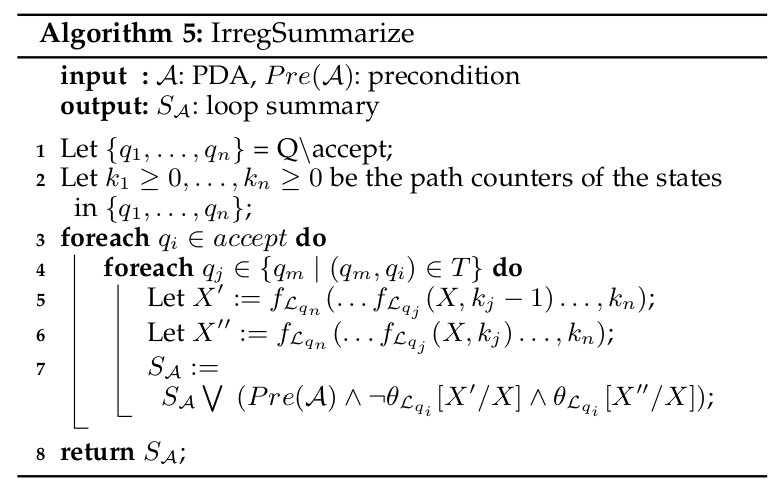
\includegraphics[scale=0.35]{algo5.png}
\end{center}
\end{frame}
\fi
\begin{frame}\frametitle{Experimental Results: Loop Bound}
\begin{center}
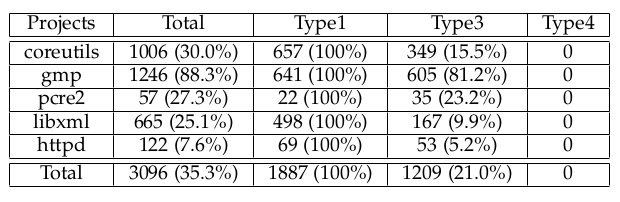
\includegraphics[scale=0.4]{loopbound.png}
\end{center}
\end{frame}

\begin{frame}\frametitle{Experimental Results: Program Verification}
\begin{center}
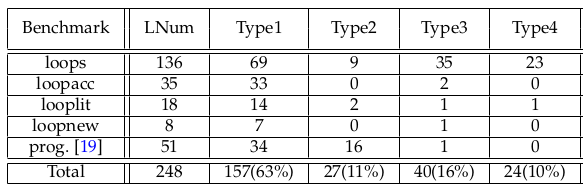
\includegraphics[scale=0.35]{loopverif.png}
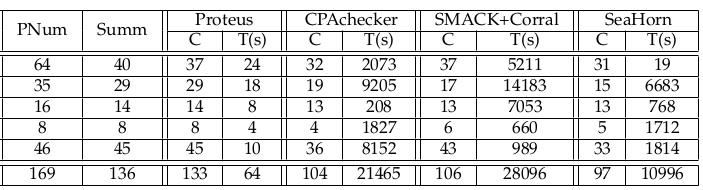
\includegraphics[scale=0.35]{loopverif1.png}
\end{center}
\end{frame}
\begin{frame}\frametitle{Experimental Results: Test Case Generation}
\begin{center}
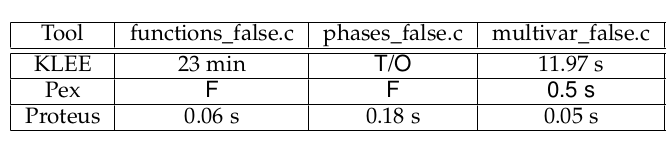
\includegraphics[scale=0.35]{testcase.png}

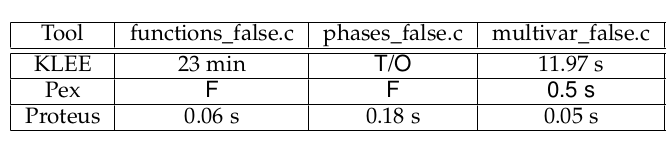
\includegraphics[scale=0.35]{testcase.png}
\end{center}
\end{frame}

\end{document}